\section{Interprocedural Analysis and Context-Sensitivity}
\subsection{Interprocedural Control Flow Graphs}
\begin{itemize}
  \item \textbf{Intraprocedural analysis} is analyzing the body of a single function
  \item \textbf{Interprocedural analysis} is analyzing the whole program with function calls
  \item The subset of the TIP language containing function is used but pointers and functions are ignored as values
  \item It is assumed that all function calls are performed in connection with assignments:
  \begin{equation*}
    X=f(E_1, \dots, E_n);
  \end{equation*}
  \item Each function call statement are represented using two nodes
  \begin{itemize}
  	\item A \textbf{call node} representing the connection from the caller to the entry of $f$
  	\item An \textbf{after-call node} where execution resumes after returning from the exit of $f$:
    \begin{figure}[H]
    	\centering
    	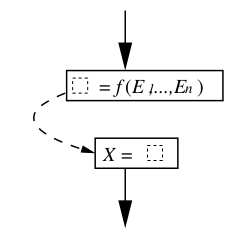
\includegraphics[width=130pt]{img/interprocedural/after_call_node}
    \end{figure}
  \end{itemize}
  \item Each $\text{return } E;$ statement are represented as an assignment using a special variable named \texttt{result}
    \begin{figure}[H]
    	\centering
    	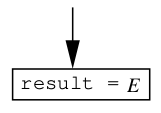
\includegraphics[width=80pt]{img/interprocedural/result}
    \end{figure}
  \item CFGs can be constructed such that there is always a unique entry node and a unique exit node for each function
  \item The caller and callee are glued together as follows:
  \begin{figure}[H]
    \centering
    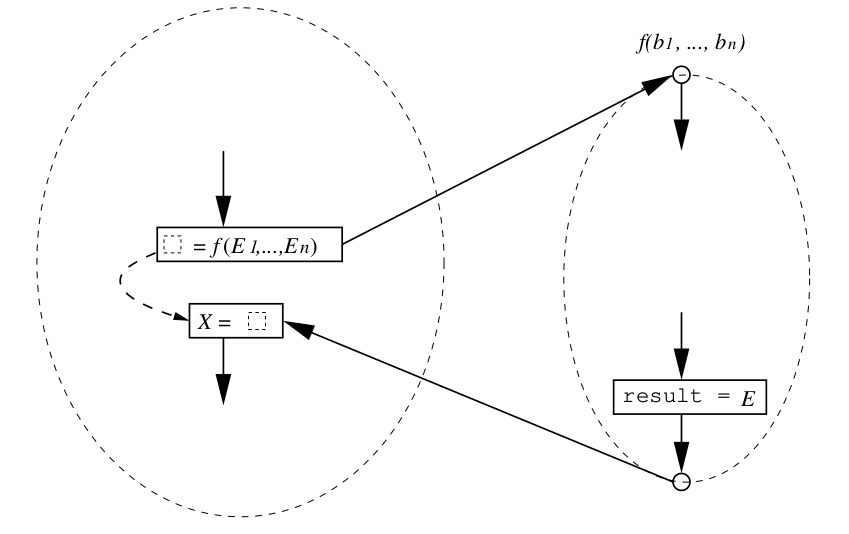
\includegraphics[width=\linewidth]{img/interprocedural/interprocedural}
  \end{figure}
  \item The connection between the call node and its after-call node is represented by a special edge, which is needed for propagating abstract values for local variables of the caller
  \item For sign analysis the interprocedural constraints can be represented as follows
  \begin{itemize}
  	\item For entry node $v$ of function $f(b_1, \dots, b_n)$ the abstract states for all callers $\text{pred}(v)$ are considered and the passing of parameters are modeled as follows
    \begin{equation*}  
      \co{v} = \bigsqcup_{w \in \text{pred}(v)} s_w
    \end{equation*}
    where
    \begin{equation*} 
      s_w = \bot[b_1 \mapsto \text{eval}(\co{w}, E_1^w), \dots, b_n \mapsto \text{eval}(\co{w}, E_n^w)]
    \end{equation*}
    where $E_i^w$ is the ith argument to the call node
    \item For the entry node $v$ of the \texttt{main} function with parameters $b_1, \dots, b_n$ 
    \begin{equation*}
      \co{v} = \bot[b_1 \mapsto \top, \dots, b_n \mapsto \top]
    \end{equation*}
    For an after-call node $v$ that stores the return value in the variable $X$ and where $v'$ is the accompanying call node and $w \in \text{pred}(v)$ is the function exit node 
    \begin{equation*}
      \co{v} = \co{v'}[X \mapsto \co{w}(\mathtt{result})]
    \end{equation*}
    \item For this analysis there are no constraints needed for call nodes and exit nodes
    \begin{itemize}
    	\item For a backward analysis one would consider the call nodes and the function exit nodes instead 
    \end{itemize}
  \end{itemize}
\end{itemize}

\subsection{Context Sensitivity}
\begin{itemize}
  \item When calling a function multiple times it can mess up the result
  \begin{itemize}
  	\item Since data is flowing along \textbf{interprocedurally invalid paths}
  \end{itemize}
  \item A simple solution to calling a function multiple times is to clone the function
  \begin{itemize}
  	\item It can also be achieved by inlinening the function
  	\item It can be achieved using context-sensitive analysis on the form
  \end{itemize}
  \begin{equation*}
    (\text{Contexts} \rightarrow \text{lift}(\text{States}))^n
  \end{equation*}
  \item The bottom element of $\text{lift}(\text{States})$, is denoted \texttt{unreachable}, is used for call context that are unreachable from the program entry
  \item A trivial choice is to let Contexts be a singleton set which is the same as a context-insensitive analysis
  \begin{itemize}
  	\item Another extreme is to pick $\text{Contexts} = \text{States}$ which gives full context sensitivity 
  \end{itemize}
  \item For example the constraint rule for assignments \texttt{X=E} in sign analysis becomes 
  \begin{equation*}
    X = E: \quad \co{v}(c) =
    \begin{cases} 
      s[X \mapsto \text{eval}(s,E)] & \text{if } s = \text{JOIN}(v,c) \in \text{States} \\
      \text{unreachable}            & \text{if } \text{JOIN}(v,c) = \text{unreachable}
    \end{cases}
  \end{equation*}
  where 
  \begin{equation*}
    \text{JOIN}(v,c) = \bigsqcup_{w \in \text{pred}(v)} \co{w}(c)
  \end{equation*}
\end{itemize}

\subsection{Context Sensitivity with Call Strings}
\begin{itemize}
  \item Let Calls be the set of call nodes in the CFG
  \item The \textbf{call string} approach to context sensitivity defines
  \begin{equation*}
    \text{Contexts} = \text{Calls}^{\leq k}
  \end{equation*}
  where $k$ is a positive integer
	\item A similar effect is obtained as function cloning or inlining without changing the CFG
  \item The idea is that a tuple $(c_1, c_2, \dots, c_m) \in Calls ^{\leq k}$ identifies the topmost $m$ call sites on the call stack
	\item If $(e_1, \dots, e_n) \in (\text{Contexts} \rightarrow \text{States})^n$ is a lattice element then $e(c_1, c_2, \dots, c_m)$ provides an abstract state that approximate runtime states that can appear at the ith CFG node
  \begin{itemize}
  	\item This is assuming that the the node was called from $c_i$ in each case
    \item The worst-case complexity of the analysis is affected by the choice of $k$
  \end{itemize}
  \item The constraint rule for an node $v$ of a function $f(b_1, \dots, b_n)$ are changed as follows where it takes the call context $c$ at the function entry into account and the call context $c'$ at each call node into account:
  \begin{equation*}
    \co{v}(c) = \bigsqcup_{\begin{aligned} w & \in \text{pred}(v) \; \land \\ & c = w \; \land \\  & c' \in \text{Contexts} \end{aligned}} s_w^{c'}
  \end{equation*}
  where $s_w^{c'}$ is the abstract state created from the call at node $w$ in context $c'$ 
  \begin{equation*}
    s_w^{c'} =
  \begin{cases} 
    \text{unreachable} & \text{if } \co{w}(c') = \text{unreachable}\\
    \bot[b_1 \mapsto \text{eval}(\co{w}(c'), E_1^w), \dots, b_n \mapsto \text{eval}(\co{w}(c'),E_n^w)] & \text{otherwise}
  \end{cases}
  \end{equation*}
  \item The constraint rule for an after-call node $v$ which stores the return value in the variable $X$ and $v'$ is the associated call node and $w \in \text{pred}(v)$ is the function exit node
  \begin{equation*}
    \co{v}(c) = 
    \begin{cases} 
      \text{unreachable} & \text{if } \co{v'}(c) = \text{unreachable} \lor \co{w}(v') = \text{unreachable} \\
      \co{v'}(c)[X \mapsto [\co{w}(v')(\mathtt{result})]] & \text{otherwise}
    \end{cases}
  \end{equation*}
  \item In practice $k = 1$ sometimes gives inadequate precision and $k \geq 2$ is generally too expensive
  \begin{itemize}
  	\item It is often a good idea to select $k$ individually for each call site based on heuristics 
  \end{itemize}
  
\end{itemize}

\subsection{Context Sensitivity with a functional approach}
\begin{itemize}
  \item In the \textbf{functional approach} it distinguishes calls based on abstract states at the calls and therefore uses
  \begin{equation*}
    \text{Context} = \text{States}
  \end{equation*}
  \item The analysis lattice becomes
  \begin{equation*}
    (\text{States} \rightarrow \text{lift}(\text{States}))^n 
  \end{equation*}	
  \item A lattice element for a CFG node $v$ is a map $m: \text{States} \rightarrow \text{lift}(\text{States})$
  \begin{itemize}
    \item Such that $m(s)$ approximates the possible states at $v$ given that the current function containing $v$ was entered in a state that matches $s$
    \item $m(s) = \text{unreachable}$ means that there is no execution of the program where the function is entered in a state that matches $s$ and $v$ reached
  \end{itemize}
  \item The constraint rule for an entry node $v$ of a function $f(b_1, \dots, b_n)$ is the same as in the call strings approach except for the condition on $c$ 
  \begin{equation*}
    \co{w}(c) = \bigsqcup_{\begin{aligned} w & \in \text{pred}(v) \; \land \\ & c = s_w^{c'} \; \land \\  & c' \in \text{Contexts} \end{aligned}} s_w^{c'}
  \end{equation*}
  \item The constraint rule for an after-call node $v$ which stores the return value in the variable $X$ and $v'$ is the associated call node and $w \in \text{pred}(v)$ is the function exit node
  \begin{equation*}
    \co{v}(c) = 
    \begin{cases} 
      \text{unreachable} & \text{if } \co{v'}(c) = \text{unreachable} \lor \co{w}(s_{v'}^c) = \text{unreachable} \\
      \co{v'}(c)[X \mapsto [\co{w}(v')(\mathtt{result})]] & \text{otherwise}
    \end{cases}
  \end{equation*}
\end{itemize}

\newpage

%%% Local Variables:
%%% mode: latex
%%% TeX-master: "pav-noter"
%%% End:
